\documentclass[11pt]{article}
\usepackage[a4paper,margin=25mm]{geometry}
\usepackage{graphicx,amsmath,amssymb,amsthm,booktabs,multirow,float}
\usepackage[T1]{fontenc}\usepackage{lmodern,microtype}
\usepackage[round,authoryear]{natbib}\usepackage{hyperref,xurl}
\input{glyphtounicode}\pdfgentounicode=1
\theoremstyle{plain}
\newtheorem{theorem}{Theorem}\newtheorem{proposition}[theorem]{Proposition}\newtheorem{lemma}[theorem]{Lemma}
\theoremstyle{definition}\newtheorem{remark}{Remark}\newtheorem{example}{Example}
\newcommand{\T}{\mathcal T}\newcommand{\Pp}{\mathbb P}\newcommand{\E}{\mathbb E}\newcommand{\ind}{\mathbf1}
\newif\ifanonymous\ifdefined\blindversion\anonymoustrue\else\anonymousfalse\fi
\newsavebox{\resultsbox}
\raggedbottom\setlength{\emergencystretch}{2em}
\hypersetup{colorlinks=true,linkcolor=black,citecolor=black,urlcolor=blue,pdftitle={Certified degree bounds and hub exclusions in correlation spanning trees}}
\title{Certified degree bounds and hub exclusions in correlation spanning trees}
\ifanonymous
\author{}\hypersetup{pdfauthor={}}
\else
\author{Marek Ga\l{}\k{a}zka\textsuperscript{1}\thanks{Corresponding author: galazka@amu.edu.pl}\quad Hanna Wdowicka\textsuperscript{2}\\[5pt]
\small\textsuperscript{1}Faculty of Mathematics and Computer Science,\\[-2pt]
\small Adam Mickiewicz University, Pozna\'n, Poland\\[3pt]
\small\textsuperscript{2}Department of Statistics, Pozna\'n University of Economics and Business, Poland}
\hypersetup{pdfauthor={Marek Galazka and Hanna Wdowicka}}
\fi
\date{}
\begin{document}
\maketitle
\begin{abstract}
Which variables can be ruled out as network hubs when the most connected variable remains uncertain? We construct simultaneous degree bounds and hub exclusions for population correlation spanning trees. Averaged matching e-values for Kendall tau-a comparisons provide finite-sample error control under independent and identically distributed (IID) sampling, including ties. Tree constraints convert these comparisons into verified integer bounds. We evaluate practical benefit through changed conclusions and measured computation, separately from interval-width reductions. In pooled Abalone data, a degree-only linear-programming stage increases hub exclusions from two to four and narrows the rank of whole weight from [1,6] to [1,3] under an explicit IID working model. It requires 16 rather than 72 LP objectives and approximately one quarter of the full projection time, with identical degree and rank bounds. Across all 192 measurement analyses, degree-only projection preserves the full rank endpoints in 188; the remaining four analyses gain six additional exclusions from pair objectives. Matched simulations retain important failures: exact procedures do not identify separated-star hubs at 1008 observations, and numerical tightening often yields no new decision. The resulting workflow makes partial conclusions explicit and reserves costly pair optimization for questions that require it.
\end{abstract}
\noindent\textbf{Keywords:} Kendall tau-a; e-values; simultaneous inference; spanning tree; U-statistics; degree rank.

\section{Introduction}
When measurements are linked by their strongest correlations, which variables can be ruled out as the centre of the network? A common summary is a spanning tree: a connected set of links with no cycles. A variable's degree is its number of links; a variable with the largest degree is a hub, and a variable with one link is a leaf. An analyst may be able to establish that some variables are leaves or cannot be hubs before identifying a single most connected variable. Such partial conclusions need statistical support because the tree is built from estimated correlations.

Our contribution combines tie-aware aggregation of evidence from observation pairings with verified bounds on these partial conclusions. The statistical construction controls simultaneous errors for every finite sample under IID sampling and eventually distinguishes every fixed positive correlation gap. The computational contribution is evaluated by the decisions it adds and the cost of obtaining them. With the E64 calibration fixed, a degree-only projection excludes two additional Abalone measurements from hub status and places whole weight within the top three, using 16 LP objectives; the further 56 ordered-pair objectives add no conclusion in this example (Figure~\ref{fig:intro}). This motivates an economical workflow centred on degrees and hub exclusions. The matching-evidence construction supplies the statistical contribution; the tree-optimization rules are classical, and their integration is assessed empirically rather than treated as a new optimization theorem.

\begin{figure}[H]\centering
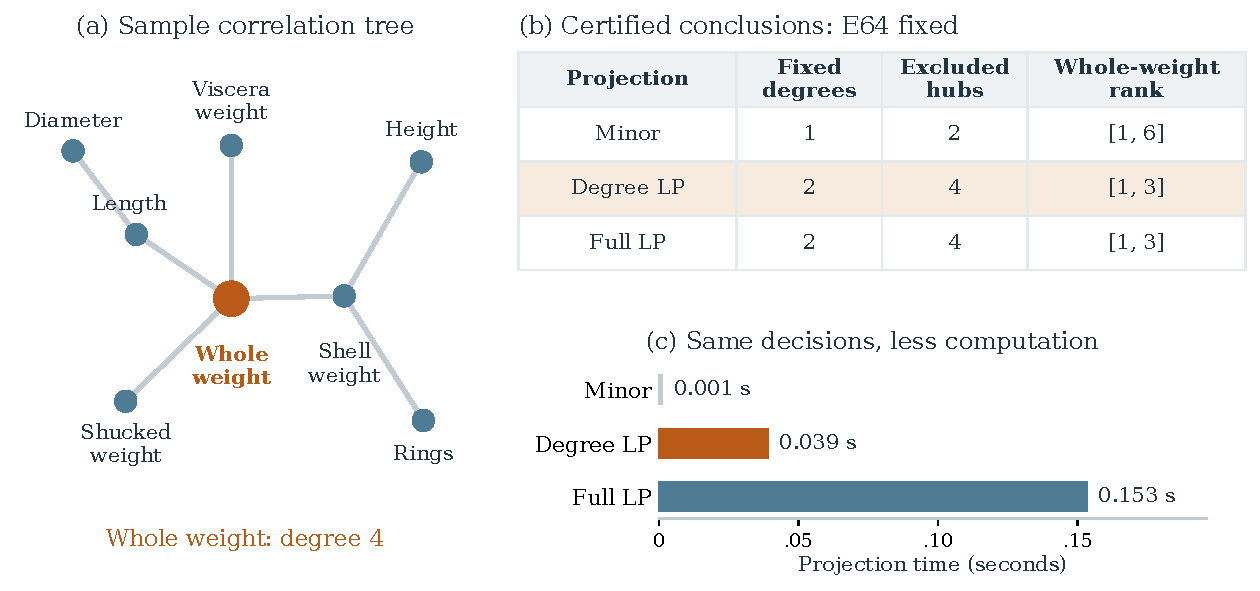
\includegraphics[width=\textwidth]{Fig_practical_abalone.pdf}
\caption{A changed conclusion and its computational cost on 4177 Abalone specimens. (a) Whole weight has four links in the sample Kendall tree. (b) Holding the E64 local-family calibration fixed, degree-only path LP certifies a second leaf, excludes two additional hubs, and narrows whole weight's rank from [1,6] to [1,3]. Full ordered-pair LP gives identical endpoints. (c) Projection times include minor construction and rational-certificate checks; medians of three controlled runs are shown. E64 calibration takes a separate 0.140 seconds. The inferential statements have simultaneous nominal confidence 95\% under the stated IID working model and cover every population-optimal tree, including degree ties. Sections~\ref{sec:decision-application} and \ref{sec:cost} give the complete decision and cost audits.}\label{fig:intro}
\end{figure}

The statistical component averages betting e-values for raw Kendall tau-a differences across matchings chosen independently of the data. A sample-size-dependent betting fraction ensures consistency for fixed positive gaps; the finite-sample expectation bound requires no moments. Conditional McNemar tests and dependence-safe p-value aggregation provide exact reference constructions. The computational component retains common-tree degree differences, adds cycle-path incompatibilities, verifies linear-programming endpoint improvements by rational weak-duality certificates, and enforces the fixed sum of tree degrees.

The cost of the exact construction is substantial: at continuous independence, a one-matching estimator has asymptotic variance 4.5 times that of the full U-statistic. We evaluate p-value aggregation over eight matchings and evidence aggregation over eight or 64 matchings, comparing these exact constructions with direct full-U-statistic Hoeffding tests and Gaussian multiplier methods. Every calibration uses the same projections. Further ablations hold tests fixed while changing rank and path projection, and compare local with complete edge families. This separates gains from calibration, use of comparisons, and feasible-tree information.

The classical foundations are important to the contribution's scope. Interval robust spanning trees and possible or necessary optimality are studied by \citet{yaman2001,kasperski2007,fortin2007}; \citet{zaffalon2005} develop robust tree inference from dependence comparisons. The cut/cycle rules, greedy matroid rank identities and weak duality used here are established optimization facts. Our contribution is the explicit tie-aware matching-evidence construction and its consistency, the integration with verified degree-difference and path projection, and a matched evaluation of the resulting inferential trade-offs. Unlike interval optimization over supplied coordinate ranges, the input is a jointly calibrated relation between population edges, followed by projection to vertex quantities. Spanning-tree sensitivity analysis supplies related algorithmic context \citep{pettie2014}.

Rank inference must retain population ties \citep{hall2009,mogstad2024}. Combinatorial inference for graphical models studies other graph properties under different structural models \citep{neykov2019}. A correlation-optimal tree is an association summary. In financial networks, bootstrap edge reliability \citep{tumminello2007,musciotto2018} and Polish market correlations \citep{galazka2011} motivate the practical comparison. Edge or hub selection frequencies and simultaneous population degree statements are distinct statistical targets.

The primary measured-data example concerns Abalone morphometrics. Whole weight is the unique sample hub in all 499 bootstrap trees, yet its exact population rank remains [1,3]. The practical gain is instead two certified leaves and four hub exclusions under an explicit cross-sectional IID working model. An audit retains all 12 measurement populations, eight calibrations and both comparison families, including analyses that produce no new decision. A controlled 50-case timing study measures the cost of each computational stage. Polish returns and the paired Pearson-bootstrap audit appear as separate diagnostic studies in the appendices.

\section{Population target and simultaneous orders}
Let $G=(V,E)$ be a fixed connected graph with $p\ge2$ vertices and $m$ edges. For weights $w$, let
\[
 \T(w)=\arg\max_{T\text{ spanning tree}}\sum_{e\in T}w_e.
\]
In the correlation application $G$ is complete. A maximum-correlation tree has the same optimal-tree family as the minimum-distance tree based on $\sqrt{2(1-w_e)}$: both are determined by the same edge ordering, including ties. Strictly increasing edge transformations preserve this family.

\paragraph{Pearson and Kendall targets.}
Gaussian and $t_5$ correlations have the same edge ordering as their Kendall weights, but this relation need not extend to a nonelliptical population. For a concrete construction, start with the $p=12$ separated Gaussian star below and set $Y_i=\exp(\sigma_i X_i)$, where $\sigma_0=2.5$ and the other scales span $[0.3,1.5]$. Monotonicity leaves every Kendall kernel unchanged. The normal exponential moment formula gives
\[
 \rho^{Y}_{ij}=\frac{\exp(\sigma_i\sigma_j\rho^X_{ij})-1}{\sqrt{(\exp(\sigma_i^2)-1)(\exp(\sigma_j^2)-1)}}.
\]
The Kendall tree has vertex-zero degree 11, whereas the Pearson tree has vertex-zero degree 1. The supplied verifier checks both population trees and kernel invariance. Thus the weight definition is part of the inferential target.

Write $S_i=\{e:i\in e\}$ and $d_i(T)=|T\cap S_i|$. Descending ranks of vertex $i$, including every resolution of equal degrees, range from
\begin{equation}\label{eq:ranks}
 r_i^-(T)=1+\sum_{j\ne i}\ind\{d_j(T)>d_i(T)\},\qquad
 r_i^+(T)=p-\sum_{j\ne i}\ind\{d_j(T)<d_i(T)\}.
\end{equation}
The inferential target contains these quantities for every $T\in\T(w_0)$. Under complete independence all edges have weight zero, every labelled tree is optimal, and the appropriate degree and rank targets are $[1,p-1]$ and $[1,p]$. Selecting one arbitrary tied optimum would artificially narrow this target.

A random strict relation $\widehat{\succ}$ is simultaneously valid if
\begin{equation}\label{eq:event}
 \Pp(\mathcal E)\ge1-\alpha,\qquad
 \mathcal E=\{e\widehat{\succ}f\Longrightarrow w_{0e}>w_{0f}\text{ for all }e,f\}.
\end{equation}
We may take its transitive closure without an additional error budget. Every computational restriction below is conditional on this same event. The relation need not specify all pairwise edge comparisons, and its incompleteness is a source of conservative bounds.

\section{An exact Kendall comparison construction}\label{sec:kendall}
Suppose $X_1,\ldots,X_n$ are IID $p$-vectors. Coordinates may be dependent or discrete, and no moment assumption is imposed. For independent copies $X,X'$, define
\[
 \tau_{ij}=\E[\operatorname{sgn}(X_i-X_i')\operatorname{sgn}(X_j-X_j')].
\]
This is Kendall tau-a, not the tie-normalized tau-b. Attach independent uniform random variables $U_{ti}$ to each observation and coordinate, and order $\widetilde X_{ti}=(X_{ti},U_{ti})$ lexicographically. Randomization is independent of the observed sample.

For a predetermined pairing $(1,2),(3,4),\ldots$, let $N=\lfloor n/2\rfloor$ and
\[
 S_{ki}=\operatorname{sgn}(\widetilde X_{2k-1,i}-\widetilde X_{2k,i}),\qquad
 H_{k,e}=S_{ki}S_{kj},\quad e=\{i,j\}.
\]
Here $H_{k,e}\in\{-1,1\}$ and the vectors $H_k$ are IID. For an ordered comparison $(e,f)$ set
\[
 \begin{aligned} A_{ef}&=\sum_k\ind\{H_{k,e}=1,H_{k,f}=-1\},\\
 B_{ef}&=\sum_k\ind\{H_{k,e}=-1,H_{k,f}=1\},\qquad D_{ef}=A_{ef}+B_{ef}.\end{aligned}
\]
The one-sided exact p-value is
\begin{equation}\label{eq:pvalue}
 p_{ef}=\Pp\{\operatorname{Bin}(D_{ef},1/2)\ge A_{ef}\},
\end{equation}
with value one when $D_{ef}=0$. This is the conditional McNemar test \citep{mcnemar1947}, applied to paired edge kernels.

For a fixed family of unordered edge pairs $\mathcal C$, we test both directions, giving $K=2|\mathcal C|$ hypotheses. The local family consists of distinct edges sharing a vertex and has $K=p(p-1)(p-2)$ on a complete graph. The complete family and its multiplicity cost are examined below. Apply Holm's step-down rule \citep{holm1979} at level $\alpha$: ordered p-values $p_{(k)}$ are rejected until the first failure of $p_{(k)}\le\alpha/(K-k+1)$. Rejections define $e\widehat{\succ}f$; subsequently take the transitive closure.

\begin{theorem}[Finite-sample order and hub coverage]\label{thm:finite}
For IID rows and the predetermined pairing above, the resulting relation satisfies \eqref{eq:event} with $w_{0e}=\tau_e$, for every finite $n\ge2$. The probability includes auxiliary tie randomization. Consequently, every degree, degree-difference and rank bound obtained by the valid outer projections in Sections~\ref{sec:minor}--\ref{sec:rank} covers its target simultaneously with probability at least $1-\alpha$, for all population-optimal trees and every resolution of degree ties.
\end{theorem}
\begin{proof}
Conditional on $X,X'$, if neither coordinate is tied, the augmented sign product equals the original sign product. If either is tied, the independent auxiliary sign for that coordinate has mean zero. Thus $\E H_{k,e}=\tau_e$, including when both coordinates tie. Put $\pi_+=\Pp(H_e=1,H_f=-1)$ and $\pi_-=\Pp(H_e=-1,H_f=1)$. Then $\tau_e-\tau_f=2(\pi_+-\pi_-)$. Conditional on $D_{ef}$, $A_{ef}$ is binomial with success probability $q=\pi_+/(\pi_++\pi_-)$ whenever the denominator is positive. Under $\tau_e\le\tau_f$, $q\le1/2$, so \eqref{eq:pvalue} is superuniform by binomial stochastic monotonicity. The zero-denominator case gives $D_{ef}=0$ almost surely. Holm's argument therefore controls the probability of any false strict order by $\alpha$, regardless of dependence among comparisons. Transitive consequences remain true on the same event. Each subsequent outer projection retains all population-optimal trees on that event, proving the final assertion.
\end{proof}

The pairing cannot be selected after inspecting which arrangement gives favorable tests. A fixed pairing, or independent random pairing, is valid; trying several and retaining the best requires additional multiplicity control. This construction deliberately uses $N$ independent pairs. The full-sample Kendall estimator uses all $n(n-1)/2$ pairs, whose kernels are dependent. Treating those kernels as independent would invalidate the binomial calculation. Applying the IID result to serially dependent financial returns or fitted residuals is also unjustified.

\begin{proposition}[A sufficient discordance-dependent power bound]\label{prop:power}
Consider $s\ge1$ selected true comparisons from the tested family. Suppose each has gap $\Delta=\tau_e-\tau_f\ge\delta>0$ and discordance probability $d=\Pp(H_e\ne H_f)\le\bar d$. If
\begin{equation}\label{eq:power}
 N\ge\frac{64\bar d}{\delta^2}\max\left\{\log\frac K\alpha,\log\frac{2s}\eta\right\},\qquad 0<\eta<1,
\end{equation}
then all these comparisons are rejected with probability at least $1-\eta$.
\end{proposition}
\begin{proof}
Let $Z_k=(H_{k,e}-H_{k,f})/2$. Its mean is $\Delta/2$, variance is at most $\bar d$, and its centered absolute value is at most two. Bernstein's inequality gives
\[
 \Pp\{A-B<N\delta/4\}
 \le \exp\{-N\delta^2/(32\bar d+16\delta/3)\}
 \le \exp\{-N\delta^2/(64\bar d)\},
\]
where $\delta\le2\bar d$. A second Bernstein bound gives $\Pp(D>2N\bar d)\le\exp(-3N\bar d/8)$. Outside these events, the binomial Hoeffding bound implies
\[
 p_{ef}\le\exp\{-(A-B)^2/(2D)\}\le\exp\{-N\delta^2/(64\bar d)\}.
\]
Put $t=N\delta^2/(64\bar d)$. Since $\delta^2\le4\bar d^2$, both bad-event probabilities are at most $e^{-t}$. Condition \eqref{eq:power} gives $e^{-t}\le\alpha/K$ and $2s e^{-t}\le\eta$. A union bound over the $s$ comparisons therefore gives the required probability, and every p-value at most $\alpha/K$ is rejected by Holm.
\end{proof}

The bound exhibits the role of discordance in simultaneous power. It is a sufficient condition; estimator efficiency and realized power are examined next.

\subsection{Efficiency and repeated independent matchings}
The disjoint-pair construction exchanges information for an exact conditional test. Randomized incomplete U-statistics offer related statistical/computational trade-offs \citep{chenkato2019}. This cost is explicit at a continuous independence model. For adjacent edges $e=\{v,a\}$ and $f=\{v,b\}$, write $h=H_e-H_f$. Then $\operatorname{Var}(h)=2$. After transforming the three margins to independent uniforms, its first-order projection is
\[
 g(U)=(2U_v-1)\{(2U_a-1)-(2U_b-1)\},\qquad
 \zeta_1=\operatorname{Var}\{g(U)\}=2/9.
\]
The paired estimator has variance $2/N\sim4/n$, while the full order-two U-statistic has asymptotic variance $4\zeta_1/n=8/(9n)$. Their variance ratio is $4.5$, corresponding to about $22\%$ relative efficiency. This calculation describes the continuous independence model; power also depends on the alternative, discordances and the simultaneous-testing family.

We therefore evaluate $R=8$ matchings, the first predetermined and the others independent uniform permutations chosen independently of the measurements. Independent auxiliary tie randomization is used in each matching. Let $p^{(r)}_{ef}$ be its unadjusted one-sided p-value and define
\begin{equation}\label{eq:merge}
 \widetilde p_{ef}=\min\left\{1,\frac{2}{R}\sum_{r=1}^R p^{(r)}_{ef}\right\}.
\end{equation}
For $R=1$ we retain the original p-value. The factor two is the dependence-safe arithmetic-mean merging rule of \citet{vovk2020}. Matchings share observations, so their p-values are dependent.

\begin{proposition}[Finite-sample validity of matching aggregation]\label{prop:merge}
Under the sampling assumptions of Theorem~\ref{thm:finite}, apply Holm to \eqref{eq:merge} over a fixed comparison family. Retain any subset of its rejections and then take transitive closure. The resulting strict orders, and every subsequent degree or rank projection, satisfy the same familywise guarantee $1-\alpha$.
\end{proposition}
\begin{proof}
Conditional on any independently chosen matching, each null p-value is superuniform by Theorem~\ref{thm:finite}. It remains superuniform after averaging over the matching randomization. The arithmetic-mean rule is valid under arbitrary dependence, so every merged null p-value is superuniform. Holm controls any false rejection. Deleting rejections cannot increase this event, and the transitive consequences of true strict orders are true.
\end{proof}
For reproducible closure, the implementation retains only merged rejections consistent with the average paired edge scores. This deletion preserves the guarantee. It does not introduce comparisons that failed Holm. Aggregating p-values reduces dependence on an individual matching, but its power must be measured: the factor two and p-value averaging can be conservative. For comparison, averaging $R$ independently randomized matching \emph{estimators} has variance $\operatorname{Var}(U)+(\operatorname{Var}(V)-\operatorname{Var}(U))/R$, by conditional expectation over matchings. At the independence model its asymptotic variance relative to the full U-statistic is $1+3.5/R$. This estimator calculation alone does not establish an equivalent efficiency for \eqref{eq:merge}.

\subsection{Exact evidence aggregation with deterministic tie handling}\label{sec:evalues}
P-value averaging can be conservative at a large comparison family. We therefore also aggregate nonnegative evidence with null expectation at most one, an e-value \citep{vovk2021}. For matching $r$, use the original tau-a kernels $K_{r,k,e}\in\{-1,0,1\}$, retaining zero at a tied coordinate, and set $Z_{r,k,ef}=(K_{r,k,e}-K_{r,k,f})/2\in[-1,1]$. For a predetermined fraction $0\le\lambda<1$, define
\[
 E_{r,\lambda,ef}=\prod_{k=1}^N(1+\lambda Z_{r,k,ef}).
\]
The evaluated multiset of seven fractions is
\[
 \Lambda_N=\{1/32,1/16,1/8,1/4,1/2,3/4,\min(1/2,N^{-1/2})\}.
\]
Its last element is determined by sample size and ensures consistency even for gaps too small for the fixed fractions. We compare $R=8$ and $R=64$ matchings, with the former nested in the latter, and put
\begin{equation}\label{eq:evalue}
 \overline E_{ef}=\frac1{7R}\sum_{r=1}^R\sum_{\lambda\in\Lambda_N}E_{r,\lambda,ef},\qquad
 p^E_{ef}=\min\{1,1/\overline E_{ef}\}.
\end{equation}
The averaging rule is classical e-value merging. Its use here combines exact Kendall contrast evidence across shared-observation matchings. The statistic handles ties directly, without auxiliary sign randomization. Matching randomization uses the same stream as the p-value comparator, with unused tie draws retained solely to align the matching sequences.

\begin{proposition}[Finite-sample evidence validity and fixed-family consistency]\label{prop:evalues}
Under IID rows, Holm applied to \eqref{eq:evalue} controls false strict orders at level $\alpha$, including discrete margins. Deleting rejections inconsistent with the full-sample Kendall scores and taking transitive closure preserves this control. For fixed $R$ and a fixed comparison family, each comparison with $\tau_e>\tau_f$ is rejected with probability tending to one as $n\to\infty$.
\end{proposition}
\begin{proof}
For a fixed independently selected matching, the contrasts $Z_k$ are IID with $\E Z_k=(\tau_e-\tau_f)/2$. Under the null this mean is nonpositive, so nonnegativity and independence give
\[
 \E E_{r,\lambda,ef}=\{1+\lambda\E Z_k\}^N\le1.
\]
Averaging over fractions and matchings preserves the expectation bound regardless of their dependence. Markov's inequality makes the reciprocal p-value superuniform. Holm, deletion and transitive closure give the common event used by all projections.

For a fixed positive gap $\Delta$, take the first matching and $\lambda_N=N^{-1/2}$ for $N\ge4$. Since $\log(1+u)\ge u-u^2$ for $|u|\le1/2$,
\[
 \log E_{1,\lambda_N,ef}\ge N^{-1/2}\sum_k Z_k-N^{-1}\sum_kZ_k^2
 \ge \sqrt N\{\Delta/2+o_{\Pp}(1)\}-1\ \longrightarrow\ \infty.
\]
Thus $\overline E_{ef}\ge E_{1,\lambda_N,ef}/(7R)$ diverges in probability, and $p^E_{ef}\to0$. The full-sample Kendall difference converges to $\Delta$, so the consistency filter retains the direction with probability tending to one. Holm's threshold is at least $\alpha/K>0$ for a fixed family, proving the assertion.
\end{proof}
The result establishes validity and consistency; relative power varies by design and is measured below. The simulations compare both evidence averages with the same eight-matching p-value pool and with full-U-statistic methods. For continuous margins and local comparisons, $H_{\{v,a\}}H_{\{v,b\}}=S_aS_b$: one $p\times p$ sign Gram matrix supplies all discordance counts in $O(Np^2+K)$ work per matching. Tied raw kernels use exact five-category contrast counts. Logarithmic accumulation prevents numerical overflow of products, while independent direct-kernel checks verify the counts and evidence calculations.

\subsection{A finite-sample comparator using all observation pairs}
Define $k_e(X_s,X_t)=\operatorname{sgn}(X_{si}-X_{ti})\operatorname{sgn}(X_{sj}-X_{tj})$ and
\[
 \widehat\tau_e={\binom n2}^{-1}\sum_{s<t} k_e(X_s,X_t),\qquad
 \widehat\Delta_{ef}=\widehat\tau_e-\widehat\tau_f.
\]
The difference kernel lies in $[-2,2]$, including ties. Hoeffding's order-two U-statistic inequality \citep{hoeffding1963} gives
\begin{equation}\label{eq:directhoeffding}
 \Pp\{\widehat\Delta_{ef}-\Delta_{ef}\ge t\}
 \le \exp(-Nt^2/8).
\end{equation}
Consequently $p^{U}_{ef}=\exp\{-N(\max\{\widehat\Delta_{ef},0\})^2/8\}$ is superuniform under $\Delta_{ef}\le0$. Holm and the same projections therefore give finite-sample simultaneous inference. To see \eqref{eq:directhoeffding} directly, average the disjoint-pair mean over a uniform random matching conditional on the sample. This conditional average is $\widehat\Delta_{ef}$. Jensen's inequality bounds its exponential moment by that of a mean of $N$ independent kernels of range four; optimizing the usual bounded-variable exponential bound gives \eqref{eq:directhoeffding}. Thus dependence between the $\binom n2$ kernels is respected.

This comparator isolates direct testing from rectangularization while retaining a finite-sample guarantee. Its bounded-range calibration can remain conservative even though its estimator uses all pairs.

\subsection{Full U-statistics with Gaussian multiplier calibration}\label{sec:multiplier}
For a computationally stronger comparator, estimate the first-order influence by
\[
 \widehat\psi_{te}=2\left\{\frac1{n-1}\sum_{s\ne t} k_e(X_s,X_t)-\widehat\tau_e\right\}.
\]
Given independent standard normal multipliers $\xi_t^{(b)}$, put $Z_e^{*(b)}=n^{-1}\sum_t\xi_t^{(b)}\widehat\psi_{te}$ and
\[
 s_{ef}^2=n^{-2}\sum_t(\widehat\psi_{te}-\widehat\psi_{tf})^2,\qquad
 Q_b=\max_{\{e,f\}\in\mathcal C}\frac{|Z_e^{*(b)}-Z_f^{*(b)}|}{s_{ef}}.
\]
The empirical $1-\alpha$ quantile $q$ gives intervals $\widehat\Delta_{ef}\pm qs_{ef}$. Intervals excluding zero supply strict orders. This is an asymptotic IID procedure for nondegenerate projections, grounded in Gaussian and multiplier approximation for high-dimensional U-statistics \citep{chen2018,cck2013}. Theorem~\ref{thm:finite} applies to the exact methods above; multiplier calibration has its own approximation assumptions. Numerically degenerate contrasts are omitted, and their counts are reported.

The matched multiplier rectangular comparator uses the same scores, influences and multiplier draws, calibrates the maximum standardized error across individual edges, and converts its edge intervals into strict orders over the same family $\mathcal C$. Both comparators then use identical tree projections. This comparison measures the effect of calibrating differences rather than separate edge weights.

Tie-safe forward and backward Fenwick sweeps compute every rowwise kernel mean in $O(p^2n\log n)$ time. Contrast maxima are streamed in C++ without allocating a $B\times|\mathcal C|$ matrix. These implementations retain the full tau-a statistic and its shared-edge covariance.

\subsection{Local and complete families}
Every fixed comparison family can be used in the exact constructions. We compare all pairs sharing a vertex with all pairs of distinct edges. Their ordered hypothesis counts on a complete graph are $K_{\rm local}=p(p-1)(p-2)$ and $K_{\rm all}=m(m-1)$, with ratio $(p+1)/4$ for $p\ge3$. At $p=52$ these are $132{,}600$ and $1{,}756{,}950$.

Complete comparisons can add nonlocal information relevant to cycle-path constraints, while also increasing the multiplicity penalty and computation. Transitive closure of local orders recovers some nonlocal comparisons, but need not recover all of them. The family ablation measures the resulting trade-off at $p=12$; both families are also evaluated on every cross-sectional application. Local testing remains an explicit computational choice for the larger simulations and the Polish sensitivity study.


\section{Projecting orders into joint degree information}\label{sec:minor}
\subsection{Classical screening and exact extrema on an outer minor}
For an edge $e=\{u,v\}$, exclude $e$ if a $u$--$v$ path consists entirely of edges certified above $e$. The cycle property rules it out of every population-optimal tree. Force $e$ if $u,v$ become disconnected after deleting $e$ and all edges certified below $e$. The resulting cut has $e$ strictly heavier than every alternative, so every optimum contains it. These sufficient screening rules define the outer family used in the subsequent projections.

Let $A$ be the allowed edges and $F$ the forced edges. On $\mathcal E$, $F$ is a forest. Contract $F$, delete excluded edges, and retain the resulting graphic matroid $M$ with rank $k=p-1-|F|$ and rank function $r$. Parallel edges and loops are permitted after contraction. Every population-optimal tree is $F\cup B$ for some base $B$ of $M$, but many bases can fail to be optimal for any compatible weights. All exactness claims below refer to this outer base family.

Write $a_i=|F\cap S_i|$ and $I_i=S_i\setminus F$ restricted to the residual ground set. The ordinary greedy rank identities give
\begin{equation}\label{eq:degree}
 \underline d_i=a_i+k-r(E_M\setminus I_i),\qquad
 \overline d_i=a_i+r(I_i).
\end{equation}
For vertices $i,j$, assign residual coefficients $c_e=\ind\{e\in S_i\}-\ind\{e\in S_j\}$, and let $P_+,P_0,P_-$ denote their level sets.

\begin{proposition}[Degree-difference extrema on the minor]\label{prop:minor}
The exact maximum and minimum of $d_i-d_j$ over the outer base family are
\begin{align}
 U_{ij}&=a_i-a_j+r(P_+)+r(P_+\cup P_0)-k,\label{eq:diffmax}\\
 L_{ij}&=a_i-a_j+k-r(P_-)-r(P_-\cup P_0).\label{eq:diffmin}
\end{align}
\end{proposition}
\begin{proof}
For a base $B$ of size $k$, $\sum_{e\in B}c_e=|B\cap P_+|+|B\cap(P_+\cup P_0)|-k$. Each intersection is bounded by the corresponding rank. A greedy base processing $P_+$ first, then $P_0$, then $P_-$ attains both bounds simultaneously, by the matroid augmentation property. This proves \eqref{eq:diffmax}. Reverse signs for \eqref{eq:diffmin}. The same argument with coefficients zero and one gives \eqref{eq:degree}.
\end{proof}

These classical matroid identities give an explicit inferential calculation: $L_{ij}>0$ certifies $d_i>d_j$ for every retained tree. Directly optimizing a difference retains a common feasible tree, whereas subtracting a marginal maximum from a marginal minimum can use incompatible trees.

\subsection{Cycle-path incompatibilities}
Individual screening can leave many jointly impossible edge configurations. Suppose $P$ is a simple path between the endpoints of $e$, and $e\widehat{\succ}f$ for some $f\in P$. Every population-optimal tree satisfies
\begin{equation}\label{eq:path}
 \sum_{g\in P}x_g\le |P|-1,
\end{equation}
where $x_g$ is its edge indicator. Indeed, a tree containing all of $P$ cannot also contain $e$; replacing $f$ by $e$ would then strictly increase its weight. Notice that the condition needs one lighter edge on the path. It is stronger than excluding only an edge that is lighter than an entire alternative path.

We use every such path of length two and additional paths from eight candidate spanning trees. Candidate priorities are generated with a fixed seed, with forced edges processed first and excluded edges omitted. For each candidate and each non-tree edge, its unique path is checked against the same certified relation. Path selection may depend on the relation without a new statistical correction: every inserted inequality is valid on $\mathcal E$. Eight is a computational design choice, not a claim that these paths exhaust the useful constraints.

The linear relaxation has $0\le x_e\le1$, $\sum_e x_e=p-1$, $\sum_{e\in S_i}x_e\ge1$, fixed forced/excluded coordinates, and the selected inequalities \eqref{eq:path}. To impose connectivity, add directed nonnegative flows, root outflow minus inflow $p-1$, and outflow minus inflow $-1$ at every other vertex. For an undirected edge $e=\{u,v\}$ impose
\[
 f_{uv}+f_{vu}\le(p-1)x_e.
\]
Every tree admits these flows by routing one unit from the root to each other vertex. Fractional solutions may remain, so this is an outer relaxation, not the convex hull of compatible optimal trees.

In the new small-graph simulations and cross-sectional applications we minimize and maximize every degree and every ordered degree difference. The larger Polish sensitivity analysis optimizes degree differences between the observed highest-degree anchor and every other vertex, retaining minor bounds for all remaining pairs. Anchor choice uses the data but all projected statements use the same event $\mathcal E$.

\subsection{Rational certificates for numerical optimization}\label{sec:dual}
A floating-point optimum should not be rounded into an inferential statement without a valid bound. Write the relaxation as $Ax\le b$, $Ex=h$, $\ell\le x\le u$, incorporating both edge and flow variables. Its coefficients and bounds are integers. For an integer objective $c$, take any rational multipliers $y\le0$ and unrestricted $z$, and put $v=c-A^\top y-E^\top z$.
\begin{proposition}[Verifiable objective bound]\label{prop:dual}
For every feasible $x$,
\begin{equation}\label{eq:dual}
 c^\top x\ge b^\top y+h^\top z+\sum_j\min\{v_j\ell_j,v_ju_j\}=:q.
\end{equation}
If the target objective is integer, $\lceil q\rceil$ is a valid lower bound. Applying the formula to $-c$ gives upper bound $\lfloor-q\rfloor$.
\end{proposition}
\begin{proof}
Expand $c^\top x=y^\top Ax+z^\top Ex+v^\top x$. The first term is at least $y^\top b$ because $y\le0$; the second equals $z^\top h$; coordinatewise minimization over the box bounds the last term. Integer rounding preserves the assertion.
\end{proof}
The implementation takes inequality multipliers from HiGHS, clips them to be nonpositive and rounds downward to multiples of $2^{-20}$. Equality multipliers are rounded to that denominator. The residual and bound are then computed with checked integer arithmetic. Empirical sparse certificates contain the numerator, denominator and multipliers for every improvement. Simulation improvements are verified during each replication, with verification counts and replication seeds archived. An independent verifier reconstructs the constraints and recomputes the bound with Python arbitrary-precision integers. Validity does not require that the numerical solution satisfy KKT equations exactly, or even that its proposed multipliers be optimal.

\section{Rank projection with degree conservation}\label{sec:rank}
Let integer degree bounds be $L_i\le d_i\le U_i$, and impose
\begin{equation}\label{eq:conserve}
 \sum_i d_i=2p-2=:D_0,\qquad d_i\ge1.
\end{equation}
We compute sharp rank endpoints over this integer box intersected with \eqref{eq:conserve}. For vertex $i$, enumerate feasible $s=d_i\in[L_i,U_i]$, so that $\sum_{j\ne i}L_j\le D_0-s\le\sum_{j\ne i}U_j$.

For the worst rank, all vertices with $L_j\ge s$ are already tied with or above $i$. Each optional vertex with $L_j<s\le U_j$ costs $s-L_j$ additional degree units to reach that threshold. Starting from all lower bounds, select the cheapest such costs within budget $D_0-s-\sum_{j\ne i}L_j$. One plus the mandatory and selected counts is the largest possible rank for that $s$.

For the best rank, vertices with $L_j>s$ necessarily outrank $i$. Without raising any additional vertex above $s$, the largest possible total for the other degrees is
\[
 C(s)=\sum_{j:L_j>s}U_j+\sum_{j:L_j\le s}\min(U_j,s).
\]
If $D_0-s>C(s)$, select the fewest additional vertices whose capacities $U_j-s>0$ cover the shortfall, taking largest capacities first. Add their count and the mandatory count to one. Minimize this best rank and maximize the worst rank over feasible $s$.

\begin{proposition}[Sharpness within the degree relaxation]\label{prop:ranks}
The threshold and capacity calculations above attain the best and worst ranks over all integer vectors satisfying the degree bounds and \eqref{eq:conserve}. On the complete graph every positive integer vector with this total is the degree sequence of a labelled tree. Sharpness need not hold for the smaller family of order-compatible or minor-compatible trees.
\end{proposition}
\begin{proof}
To make $k$ optional competitors reach $s$, their required increases have minimum total equal to the sum of the $k$ smallest costs. The budget criterion is therefore necessary and sufficient; remaining degree units can be allocated within the original upper bounds. If this forced another optional competitor to reach $s$, that competitor would already have been affordable, contradicting maximality. For the best rank, activating a vertex above $s$ supplies at most $U_j-s$ additional units. The largest-capacity rule minimizes the number required. Feasibility of $s$ guarantees enough total capacity, and integer intervals allow filling the remaining total without gaps. Finally, a Pr\"ufer sequence containing vertex $i$ exactly $d_i-1$ times realizes any positive vector summing to $2p-2$.
\end{proof}

Intersect these rank intervals with direct comparison bounds
\begin{equation}\label{eq:pairranks}
 1+\#\{j:L_{ji}>0\}\ \le r_i\le\ p-\#\{j:L_{ij}>0\}.
\end{equation}
A certified unique hub has upper rank one. A vertex remains a possible hub whenever its lower rank is one. Estimated degrees are reported separately from these tie-inclusive inferential ranges. The proof of Theorem~\ref{thm:finite} now follows through every computational stage.

\subsection{Projection for a stated decision}\label{sec:decision-workflow}
For a fixed calibration and comparison family, the reported bounds answer four concrete questions: a degree is determined when $L_i=U_i$; a vertex is a leaf when $U_i=1$; hub status is excluded when the lower rank exceeds one; and membership among the top three is certified when the upper rank is at most three. A strict degree comparison also follows whenever $\max\{\underline\Delta_{ij},L_i-U_j\}>0$, where $\underline\Delta_{ij}$ is a certified lower bound on $d_i-d_j$.

The economical workflow first computes the screened minor and its pair/conservation rank bounds. If the relevant question remains unresolved, it adds the $2p$ individual degree LP objectives and recomputes ranks, retaining the minor's degree-difference bounds. The optional full stage adds $p(p-1)$ ordered-pair objectives on the same LP constraints. The degree-only and full stages therefore have the same individual degree objectives and bounds; any further inferential benefit must come through degree differences and ranks. This is an objective-selection rule, not a different confidence calibration.

All retained bounds are valid on the same event $\mathcal E$. Omitting objectives or stopping after a question has been answered can weaken the conclusions but cannot invalidate them. Thus a choice of computational effort based on the already calibrated relation needs no further error budget. Choosing whichever of several statistical calibrations gives a preferred conclusion would be a different selection problem; each reported 95\% analysis here fixes its calibration and family separately. The empirical audit below records both changed decisions and unresolved questions.

\section{A positive-definite example of lost joint information}\label{sec:example}
Consider eight vertices indexed $0,\ldots,7$. In the block $\{0,\ldots,5\}$ let hub correlations be $\rho_{0j}=0.06+t$ for $1\le j\le5$, and leaf correlations $\rho_{ij}=0.04+t$ for $1\le i<j\le5$. Set $\rho_{06}=0.10$, $\rho_{67}=0.15$, all other cross-block correlations to zero, and diagonal entries to one, with $t\in[-0.025,0.025]$.

Every matrix is positive definite: it is symmetric, has positive diagonal and is strictly diagonally dominant; the largest absolute off-diagonal row sum is $0.525$. Every within-block spoke exceeds every within-block leaf edge by $0.02$. The unique optimal tree throughout the curve consists of five spokes, the bridge $06$ and edge $67$. Its degree vector is $(6,1,1,1,1,1,2,1)$, so vertex zero is uniquely first.

Now transform correlations by Fisher's $\operatorname{atanh}$ and subtract the mean across all 28 edges at each $t$. Form the smallest coordinatewise rectangular hull of this centered curve. Global centering removes a common shift across all edges but not a shift restricted to one block. Exact rectangular projection yields degree ranges
\[
 [2,6],\ [1,5]\ (\text{each of five leaves}),\ [2,2],\ [1,1].
\]
The marginal rank construction gives vertex zero $[1,7]$. In contrast, the true local orders along the coupled curve force all seven tree edges and rank $[1,1]$. For a changing edge, the derivative of its centered Fisher weight is bounded below by $1-15/[28(1-0.085^2)]>0$; for a constant edge it is negative. Thus its coordinate extrema occur at the two endpoints. An executable verification is supplied with the code. This is a deterministic comparison of uncertainty-set shapes, not a claim that this curve is an estimated confidence region. It shows why rectangularization can discard relevant information even when the candidate matrices are positive definite and global centering has already been used.

\section{Matched simulation comparisons}\label{sec:simulation}
\subsection{Models, targets and calibration}
We evaluate eight calibrations on identical data: one-matching exact McNemar--Holm, eight-matching p-value aggregation, evidence aggregation over eight or 64 matchings, direct full-U-statistic Hoeffding--Holm, the full-sample rectangular Hoeffding comparator, Gaussian multiplier contrasts, and Gaussian multiplier edge rectangles. The rectangular methods produce orders over the same fixed family as their direct comparators, and every method passes through the same projections.

For the separated Gaussian model, $X_i=a_i Z+\sqrt{1-a_i^2}\epsilon_i$, with independent standard normals, $a_0=0.99$ and the other loadings equally spaced over $[0.45,0.55]$. The near-tie model uses $a_0=0.8+0.5/\sqrt n$, $a_1=0.8$, with other loadings in $[0.45,0.55]$. The $t_5$ model divides each Gaussian row by an independent $\sqrt{\chi_5^2/5}$. These models have a unique population star centred at zero; their population Kendall weights equal $2\arcsin(\rho)/\pi$.

Gaussian independence and IID uniform coordinates on $\{-1,0,1\}$ evaluate null comparisons and exact ties. Every labelled tree is optimal in these null models, so coverage must include degree ranges $[1,p-1]$ and rank ranges $[1,p]$, rather than the degrees of one tie-broken tree. Two additional Gaussian tree models avoid restricting the comparison to a uniquely dominant star. The chain has parent correlation $0.75$; the two-hub model has bridge correlation $0.5$ and leaf-parent correlation $0.7$, with five leaves attached to each hub at $p=12$. All population tree edges are unique optima, but equal vertex degrees retain their full tied rank ranges.

The 24 cells comprise 7,800 independent datasets. At $p=12$, the three star designs use $n\in\{252,1008,4096\}$ and 200 datasets per cell. At $p=52$, they use $n\in\{252,4096\}$ and 100 per cell. Gaussian null cells at $p=12$ use all three sizes, and at $p=52$ use $n=1008$; the discrete null uses $p=12,n=1008$. Every null cell has 1,000 datasets. Chain and two-hub cells use $p=12,n\in\{1008,4096\}$ and 100 datasets per cell. All tests use $\alpha=0.05$, and multiplier calibration uses 999 draws. Seeds, complete cell definitions and individual outcomes are archived.

We report false-order FWER, simultaneous degree and rank coverage, interval widths, forced edges, possible hubs and unique-hub declarations. Wilson intervals quantify Monte Carlo uncertainty. With 1,000 repetitions, the Monte Carlo standard error at probability $0.05$ is about $0.007$. A single empirical rejection proportion is not interpreted as a proof or disproof of a coverage theorem.

\subsection{Test, projection and family ablations}
For every test we compare marginal rank projection, direct degree-difference projection, degree conservation, and their intersection, using the same screened minor. This isolates computational changes from statistical calibration. For the first 100 datasets in every $p=12$ cell, we also add the cycle-path LP and optimize all ordered degree differences, rather than only anchor differences. Improvements are checked independently with Python arbitrary-precision integers. Empty order relations and a forced single tree have known sharp endpoints, so redundant LP solves are skipped. Path-stage estimates therefore have 100 repetitions per cell and are compared with the corresponding paired subset of the other stages.

The complete-edge comparison family is evaluated on the same first 100 non-null datasets in each $p=12$ cell. All four $p=12$ null cells extend both families to 1,000 datasets. Comparisons of families use matched subsets; differences in reported means do not arise from different simulated samples.

\subsection{A frequency reference from practice}
Bootstrap edge reliability is widely used in correlation networks \citep{tumminello2007,musciotto2018}. On the same $p=12$ separated-star, near-tie and Gaussian-null samples with $n=1008$ and $4096$, we compute 499 ordinary Pearson row-bootstrap trees. Pearson and Kendall have the same population optimal-tree ordering in these Gaussian designs. We record edge selection frequencies and the frequency with which the observed anchor is the unique highest-degree vertex. A threshold of $0.95$ is evaluated as a practical declaration rule, including its false hub and false forced-edge rates. It is a frequency heuristic, not a simultaneous confidence procedure. This reference uses all 200 non-null and all 1,000 null datasets in the six selected cells.

\subsection{Calibration and power results}
Table~\ref{tab:nullnew} reports null FWER for the common minor-plus-joint-rank projection. Exact methods have their finite-sample guarantee; the multiplier methods are evaluated empirically. All cellwise Wilson intervals, simultaneous coverage outcomes and replication records accompany the article.
\begin{table}[htbp]\centering\small
\setlength{\tabcolsep}{4pt}
\caption{False-order FWER at nominal 0.05; 1,000 datasets in each null cell. P: one-matching exact; M8: merged p-values; E8/E64: evidence aggregation over 8/64 matchings; M-C: multiplier contrasts; M-B: multiplier rectangle. Both Hoeffding controls have zero false orders in these cells. All methods use the local family.}\label{tab:nullnew}
\begin{lrbox}{\resultsbox}\begin{tabular}{lrrrrrr}
\toprule
Model, $p$, $n$ & P & M8 & E8 & E64 & M-C & M-B\\
\midrule
Gaussian null, 12, 252 & 0.024 & 0.000 & 0.000 & 0.001 & 0.072 & 0.002\\
Gaussian null, 12, 1008 & 0.029 & 0.000 & 0.000 & 0.000 & 0.062 & 0.003\\
Gaussian null, 12, 4096 & 0.032 & 0.000 & 0.001 & 0.000 & 0.042 & 0.001\\
Discrete null, 12, 1008 & 0.029 & 0.000 & 0.001 & 0.000 & 0.050 & 0.001\\
Gaussian null, 52, 1008 & 0.035 & 0.000 & 0.000 & 0.000 & 0.077 & 0.000\\
\bottomrule\end{tabular}\end{lrbox}\ifdim\wd\resultsbox>\linewidth\resizebox{\linewidth}{!}{\usebox{\resultsbox}}\else\usebox{\resultsbox}\fi\end{table}
The largest one-matching null estimate is 0.035, with an individual Wilson interval [0.025,0.048] (Gaussian null, $p=52$, $n=1008$). This is a cellwise Monte Carlo summary; simultaneous calibration is established by the exact-test argument.
\begin{table}[htbp]\centering\small
\setlength{\tabcolsep}{4pt}
\caption{Probability of declaring the true unique hub using the same minor and joint-rank projection. Local comparisons; 200 repetitions for the displayed $p=12$ star cells and 100 for $p=52$. Both Hoeffding controls declare no unique hub in these star cells; full results are archived. Path projection is evaluated separately on paired subsets.}\label{tab:powernew}
\begin{lrbox}{\resultsbox}\begin{tabular}{lrrrrrr}
\toprule
Model, $p$, $n$ & P & M8 & E8 & E64 & M-C & M-B\\
\midrule
Gaussian star, 12, 1008 & 0.000 & 0.000 & 0.000 & 0.000 & 1.000 & 0.900\\
Gaussian star, 12, 4096 & 1.000 & 0.990 & 1.000 & 1.000 & 1.000 & 1.000\\
$t_5$ star, 12, 1008 & 0.000 & 0.000 & 0.000 & 0.000 & 1.000 & 0.195\\
$t_5$ star, 12, 4096 & 1.000 & 1.000 & 1.000 & 1.000 & 1.000 & 1.000\\
Gaussian star, 52, 4096 & 0.670 & 0.000 & 1.000 & 1.000 & 1.000 & 1.000\\
$t_5$ star, 52, 4096 & 0.720 & 0.000 & 1.000 & 1.000 & 1.000 & 1.000\\
Near-tie star, 12, 4096 & 0.000 & 0.000 & 0.000 & 0.000 & 0.000 & 0.000\\
Near-tie star, 52, 4096 & 0.000 & 0.000 & 0.000 & 0.000 & 0.000 & 0.000\\
\bottomrule\end{tabular}\end{lrbox}\ifdim\wd\resultsbox>\linewidth\resizebox{\linewidth}{!}{\usebox{\resultsbox}}\else\usebox{\resultsbox}\fi\end{table}
Power is interpreted jointly with FWER. The multiplier contrast procedure exceeds nominal error in some IID null cells; higher declaration rates in those regimes do not establish valid superiority. The exact evidence methods provide a comparison whose error guarantee does not rely on the Gaussian approximation.
Figure~\ref{fig:powernew} compares the full sample-size grids. The merged rule is assessed as an exact alternative, rather than assumed to recover U-statistic efficiency. The bounded-range U-statistic comparator shows whether using all pairs alone is sufficient; the matched multiplier rectangle and contrast procedures isolate the effect of shared-edge covariance and direct calibration.
\begin{figure}[htbp]\centering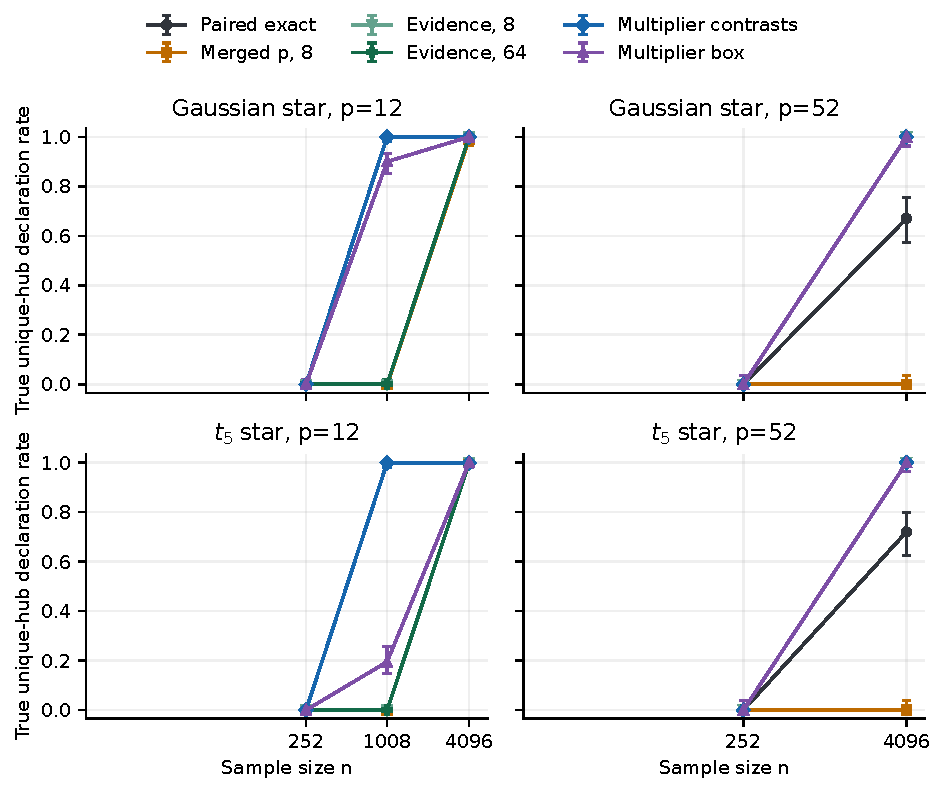
\includegraphics[width=\textwidth]{Fig_comparative.pdf}
\caption{Unique-hub declarations under the common joint projection. Curves use matched data; intervals are individual 95\% Wilson Monte Carlo intervals. All specified sample sizes and both separated distributions are shown.}\label{fig:powernew}\end{figure}
\subsection{Projection ablation}
\begin{table}[htbp]\centering\small
\setlength{\tabcolsep}{4pt}
\caption{Paired projection ablation at $p=12,n=1008$, using the same first 100 datasets per cell. Degree widths compare the minor with path LP. Rank widths compare marginal, joint pair/conservation and path projection. Complete results for all eight tests and sizes are archived. Width is upper minus lower endpoint.}\label{tab:ablation}
\begin{lrbox}{\resultsbox}\begin{tabular}{llrrrrr}
\toprule
Model & Test & $W_d$ minor & $W_d$ path & $W_r$ marg. & $W_r$ joint & $W_r$ path\\
\midrule
Gaussian star & P & 8.94 & 8.40 & 11.00 & 11.00 & 11.00\\
Gaussian star & E64 & 9.02 & 8.33 & 11.00 & 11.00 & 11.00\\
Gaussian star & M-C & 0.00 & 0.00 & 9.17 & 9.17 & 9.17\\
Near-tie star & P & 9.92 & 9.45 & 11.00 & 11.00 & 11.00\\
Near-tie star & E64 & 9.99 & 9.51 & 11.00 & 11.00 & 11.00\\
Near-tie star & M-C & 3.93 & 3.54 & 11.00 & 10.90 & 10.81\\
Chain & P & 8.00 & 4.58 & 11.00 & 11.00 & 11.00\\
Chain & E64 & 6.48 & 3.97 & 11.00 & 10.99 & 10.99\\
Chain & M-C & 0.00 & 0.00 & 7.67 & 7.67 & 7.67\\
Two hubs & P & 8.43 & 6.66 & 11.00 & 10.96 & 10.96\\
Two hubs & E64 & 5.82 & 5.11 & 10.98 & 10.54 & 10.54\\
Two hubs & M-C & 0.58 & 0.58 & 7.67 & 7.67 & 7.67\\
\bottomrule\end{tabular}\end{lrbox}\ifdim\wd\resultsbox>\linewidth\resizebox{\linewidth}{!}{\usebox{\resultsbox}}\else\usebox{\resultsbox}\fi\end{table}
The local-family path stage solves 950{,}820 LP objectives and independently verifies 375{,}946 improving rational certificates. The paired subsets show the contribution of path restrictions after fixing calibration. Degree-conservation and direct-pair rank results are additionally recorded as separate stages.
\subsection{Comparison-family ablation}
\begin{table}[htbp]\centering\small
\setlength{\tabcolsep}{4pt}
\caption{Matched local/complete family ablation at $p=12,n=4096$, 100 datasets per cell. Closed-order counts use the same $m(m-1)$ potential ordered pairs in either family. More tested comparisons also incur a larger multiplicity penalty.}\label{tab:family}
\begin{lrbox}{\resultsbox}\begin{tabular}{llrrrrrr}
\toprule
Model & Test & Orders L & Orders A & $W_d$ L & $W_d$ A & $W_r$ L & $W_r$ A\\
\midrule
Gaussian star & P & 113.0 & 530.7 & 0.14 & 0.25 & 9.17 & 9.17\\
Gaussian star & E64 & 110.8 & 579.0 & 0.00 & 0.00 & 9.17 & 9.17\\
Gaussian star & M-C & 214.4 & 643.0 & 0.00 & 0.00 & 9.17 & 9.17\\
$t_5$ star & P & 112.0 & 527.8 & 0.17 & 0.31 & 9.17 & 9.17\\
$t_5$ star & E64 & 110.5 & 573.7 & 0.00 & 0.00 & 9.17 & 9.17\\
$t_5$ star & M-C & 193.3 & 629.0 & 0.00 & 0.00 & 9.17 & 9.17\\
Near-tie star & P & 137.3 & 331.6 & 6.40 & 7.20 & 11.00 & 11.00\\
Near-tie star & E64 & 170.8 & 393.1 & 5.53 & 6.54 & 10.99 & 11.00\\
Near-tie star & M-C & 331.1 & 969.4 & 1.66 & 1.67 & 10.16 & 10.17\\
Chain & P & 850.2 & 1338.6 & 0.14 & 0.00 & 7.98 & 7.67\\
Chain & E64 & 923.0 & 1396.0 & 0.00 & 0.00 & 7.67 & 7.67\\
Chain & M-C & 1374.2 & 1766.2 & 0.00 & 0.00 & 7.67 & 7.67\\
Two hubs & P & 624.1 & 1117.3 & 0.99 & 0.38 & 7.67 & 7.67\\
Two hubs & E64 & 659.5 & 1157.1 & 0.97 & 0.02 & 7.67 & 7.67\\
Two hubs & M-C & 725.3 & 1538.1 & 0.00 & 0.00 & 7.67 & 7.67\\
\bottomrule\end{tabular}\end{lrbox}\ifdim\wd\resultsbox>\linewidth\resizebox{\linewidth}{!}{\usebox{\resultsbox}}\else\usebox{\resultsbox}\fi\end{table}
\begin{table}[htbp]\centering\small
\setlength{\tabcolsep}{4pt}
\caption{Practical row-bootstrap frequency rule on matched Gaussian samples, $p=12$, 499 draws. Hub declarations require unique-hub frequency at least 0.95; edge declarations require selection frequency at least 0.95. False edge declarations are familywise events. Frequencies have no general confidence guarantee.}\label{tab:frequency}
\begin{lrbox}{\resultsbox}\begin{tabular}{lrrrrr}
\toprule
Model & $n$ & $R$ & True hub & False hub & False edge\\
\midrule
Gaussian star & 1008 & 200 & 1.000 & 0.000 & 0.000\\
Gaussian star & 4096 & 200 & 1.000 & 0.000 & 0.000\\
Gaussian null & 1008 & 1000 & -- & 0.000 & 0.043\\
Gaussian null & 4096 & 1000 & -- & 0.000 & 0.049\\
Near-tie star & 1008 & 200 & 0.020 & 0.000 & 0.220\\
Near-tie star & 4096 & 200 & 0.060 & 0.000 & 0.225\\
\bottomrule\end{tabular}\end{lrbox}\ifdim\wd\resultsbox>\linewidth\resizebox{\linewidth}{!}{\usebox{\resultsbox}}\else\usebox{\resultsbox}\fi\end{table}
The frequency reference targets estimated-tree stability. Under the Gaussian null every edge can occur in an optimal population tree, but none is necessary and no vertex is a population unique hub. A high-frequency edge declaration is therefore counted as false necessity in that setting. This definition avoids interpreting frequent selection as a simultaneous population certificate.

\subsection{Decisions gained on the same simulated samples}\label{sec:decision-simulation}
An interval-width reduction is useful for a given question only if it changes the answer or the degree range relevant to that question. We therefore separately count fixed degrees, exclusions from hub status and unique-hub declarations. Table~\ref{tab:decision-simulation} uses the same first 100 samples for both projections and retains every non-null $p=12$ model at $n=1008$ and $4096$. The archived audit includes all 17 $p=12$ cells, both families and all eight calibrations, giving 27,200 paired method--family--dataset comparisons. These are repeated analyses of the original datasets, not new independent samples.


\begin{table}[H]\centering\small
\setlength{\tabcolsep}{4pt}
\caption{Paired E64 decision yield, local family, $p=12$. Fixed degrees and hub exclusions are mean counts per dataset before (M: minor with pair/conservation ranks) and after full path projection (F). The last column counts datasets gaining a fixed degree, a hub exclusion or a unique-hub declaration. Each row contains the same 100 samples in both stages.}\label{tab:decision-simulation}
\begin{lrbox}{\resultsbox}\begin{tabular}{llrrrrr}
\toprule
Model & $n$ & Fixed M & Fixed F & Excluded M & Excluded F & Any gain\\
\midrule
Gaussian star & 1008 & 0.00 & 0.00 & 0.00 & 0.00 & 0/100\\
Gaussian star & 4096 & 12.00 & 12.00 & 11.00 & 11.00 & 0/100\\
$t_5$ star & 1008 & 0.00 & 0.00 & 0.00 & 0.00 & 0/100\\
$t_5$ star & 4096 & 12.00 & 12.00 & 11.00 & 11.00 & 0/100\\
Near tie & 1008 & 0.00 & 0.00 & 0.00 & 0.00 & 0/100\\
Near tie & 4096 & 0.06 & 0.21 & 0.06 & 0.21 & 13/100\\
Chain & 1008 & 0.00 & 0.00 & 0.00 & 0.00 & 0/100\\
Chain & 4096 & 12.00 & 12.00 & 2.00 & 2.00 & 0/100\\
Two hubs & 1008 & 0.00 & 0.00 & 0.12 & 0.16 & 1/100\\
Two hubs & 4096 & 0.40 & 0.40 & 10.00 & 10.00 & 0/100\\
\bottomrule\end{tabular}\end{lrbox}\ifdim\wd\resultsbox>\linewidth\resizebox{\linewidth}{!}{\usebox{\resultsbox}}\else\usebox{\resultsbox}\fi\end{table}


At $n=1008$, neither exact star experiment yields a fixed degree or a hub exclusion, even after full projection. For the chain, degree width falls from $6.477$ to $3.968$ without changing these decisions. For near ties at $n=4096$, projection produces a new decision in 13 of 100 samples: the mean number of fixed degrees and excluded hubs both increase from $0.06$ to $0.21$, but no unique hub is identified. The two-hub model at $n=1008$ gains exclusions in one of 100 samples. At $n=4096$, separated-star hubs are already identified by the minor stage; the additional LP work does not create that success. Thus the exact method's larger-sample power comes primarily from calibrated edge evidence, while projection has selective value for partial decisions. Full cellwise counts and original coverage results accompany the article.


\section{Cross-sectional morphometric applications}\label{sec:crosssection}
\subsection{Recorded measurements and sampling scope}
The primary application uses all 4,177 specimens in the UCI Abalone dataset \citep{abalone1994}. Vertices are its eight numerical measurements: length, diameter, height, whole weight, shucked weight, viscera weight, shell weight and ring count. The recorded sex/status field defines three additional reported strata (female, male and infant). Original supplied measurements are retained, including zero heights and tied ring counts; no outlier removal, imputation or residual fitting is performed. The supplied complete-case dataset has no identical full rows. One independently generated permutation fixes the observation ordering before disjoint pairing.

The sampling model treats specimens as independent observations from one common distribution within each analysed population. This is a working model for cross-sectional measurements. The repository does not provide specimen identifiers, sampling clusters or acquisition batches sufficient to establish independence from the files alone. Pooled and sex-stratified results are all reported, and heterogeneity across strata is examined explicitly. The finite-sample guarantee is conditional on this IID sampling model. The nominal error level applies within one stated method and comparison family, not jointly across all reported analyses.

As a secondary computational stress study, we apply all methods to the 16 image-derived features of UCI Dry Bean, pooled and separately for all seven varieties \citep{drybean2020}. This file contains 68 repeated full rows and several mechanically related shape measurements. We retain them and report ties and degenerate contrasts. These cases assess projection and tie handling; their sampling design is insufficiently documented for an unconditional population confidence interpretation. Morphometric correlation trees describe association among measurements, including measurement identities, rather than causal or conditional-independence networks.

\subsection{Exact, merged and multiplier outputs}
All eight methods and both comparison families are applied to all 12 datasets. Every projection includes all degree and ordered degree-difference LP objectives, with independent rational verification of improvements. Ordinary row-bootstrap Kendall trees, using 499 resamples and the complete tau-a statistic, supply edge frequencies and unique-hub frequencies on the same data. These frequencies remain separate from the exact confidence statements. Original datasets are redistributed under their CC BY 4.0 licences, with source citations and unchanged-file hashes.

\begin{table}[htbp]\centering\small
\setlength{\tabcolsep}{4pt}
\caption{Primary Abalone application, $n=4177,p=8$, local family. P, M8, E8, E64, U-H and B-H have finite-sample guarantees under the stated IID sampling model; M-C and M-B use asymptotic multiplier calibration. All methods receive the same full degree-pair path projection.}\label{tab:abalone}
\begin{lrbox}{\resultsbox}\begin{tabular}{lrrrrrrr}
\toprule
Test & Orders & Forced & Fixed degrees & Hubs & $W_d$ minor & $W_d$ path & $W_r$\\
\midrule
P & 104 & 0 & 1 & 0 & 3.250 & 2.625 & 6.750\\
M8 & 89 & 0 & 0 & 0 & 4.250 & 3.250 & 7.000\\
E8 & 109 & 3 & 1 & 0 & 2.125 & 1.875 & 6.500\\
E64 & 111 & 3 & 2 & 0 & 1.875 & 1.375 & 5.625\\
U-H & 42 & 0 & 0 & 0 & 6.000 & 5.500 & 7.000\\
B-H & 45 & 0 & 0 & 0 & 6.000 & 5.250 & 7.000\\
M-C & 152 & 6 & 6 & 1 & 0.250 & 0.250 & 3.250\\
M-B & 125 & 4 & 3 & 1 & 0.875 & 0.750 & 4.875\\
\bottomrule\end{tabular}\end{lrbox}\ifdim\wd\resultsbox>\linewidth\resizebox{\linewidth}{!}{\usebox{\resultsbox}}\else\usebox{\resultsbox}\fi\end{table}
For the single-matching exact reference, path projection reduces mean degree width from 3.250 to 2.625 (19.2\%). Ring count has degree [1,1] and rank [3,8], excluding hub status under the stated model. Whole weight appears as the unique sample hub in all 499 ordinary Kendall bootstrap trees, but its one-matching exact rank remains [1,8]. The multiplier-contrast projection instead gives whole-weight degree [4,4] and rank [1,1]. This nominal bootstrap declaration and the exact confidence output are reported separately.
The estimated Pearson and Kendall Abalone trees share 5 of seven edges. Both weight definitions and all edge frequencies are archived. Their agreement in this dataset does not make the population targets interchangeable outside models with a common monotone correlation ordering. Pooled and sex-stratified results, every complete-family comparison, and all Dry Bean stress outputs are supplied without selecting favorable strata.
The exact E64 construction gives whole-weight degree [3,5] and rank [1,3], excluding 4 of the eight vertices from hub status. Its mean degree width is 1.375, 47.6\% below the single-matching exact result after the same projection. It retains a finite-sample guarantee under the same sampling model; unique-hub identification and a top-three rank restriction are distinct conclusions.
\begin{figure}[!ht]\centering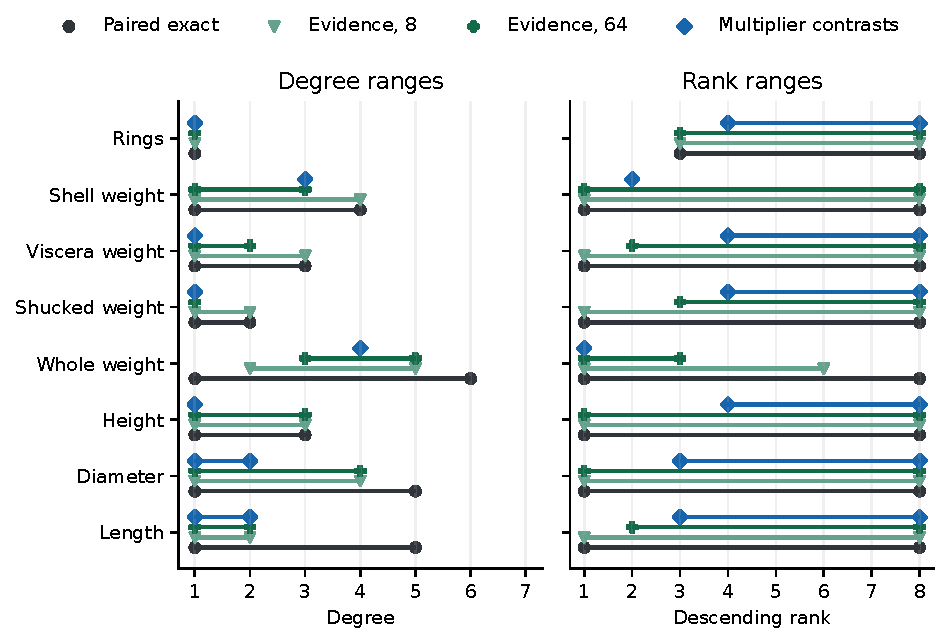
\includegraphics[width=\textwidth]{Fig_cross_section.pdf}
\caption{All eight Abalone degree and rank ranges after identical path projection. P, E8 and E64 have finite-sample guarantees under the stated IID model; M-C has asymptotic multiplier calibration. Population degree ties retain their full rank ranges.}\label{fig:cross}\end{figure}

\subsection{Which conclusions change after projection?}\label{sec:decision-application}
The primary question is which measurements can be certified as leaves, excluded from hub status, or placed within the top three. These are statements about the marginal association tree; leaf status alone does not justify removing a measurement from a predictive model. Table~\ref{tab:decision-abalone} separates the gain from replacing one matching by E64 from the gain due to subsequent optimization.


\begin{table}[H]\centering\small
\setlength{\tabcolsep}{4pt}
\caption{Abalone pooled: concrete conclusions under the IID working model and a separately chosen calibration. All rows use local edge comparisons. Fixed and excluded denote counts among eight measurements. The last two columns concern whole weight. P is one-matching exact McNemar--Holm.}\label{tab:decision-abalone}
\begin{lrbox}{\resultsbox}\begin{tabular}{llrrrr}
\toprule
Test & Projection & Fixed & Excluded & Degree & Rank\\
\midrule
P & Full LP & 1 & 1 & [1,6] & [1,8]\\
E64 & Minor & 1 & 2 & [2,5] & [1,6]\\
E64 & Degree LP & 2 & 4 & [3,5] & [1,3]\\
E64 & Full LP & 2 & 4 & [3,5] & [1,3]\\
\bottomrule\end{tabular}\end{lrbox}\ifdim\wd\resultsbox>\linewidth\resizebox{\linewidth}{!}{\usebox{\resultsbox}}\else\usebox{\resultsbox}\fi\end{table}


With E64 fixed, the minor stage excludes length and shucked weight from hub status. Degree-only path projection additionally excludes viscera weight and ring count, certifies ring count as a leaf, and raises the lower degree of whole weight from two to three. Together with degree conservation, these statements place whole weight within the top three. It is certified to have strictly greater degree than length, shucked weight, viscera weight and ring count in every population-optimal tree. The extra 56 ordered-pair LP objectives change none of the reported degree or rank endpoints. The top-three statement has a simple structural explanation. The eight degrees sum to 14. If whole weight and three competitors each had degree at least three, these four vertices plus the four remaining positive degrees would sum to at least 16. At most two competitors can therefore match or exceed whole weight. The inferential conclusion is four excluded hubs and a top-three restriction, with the identity of a unique population hub still unresolved.

Table~\ref{tab:decision-populations} reports the entire E64 local-family measurement grid, including cases with no new decision. At $n=1307$ and $1528$, degree LP certifies ring count as a leaf in the female and male Abalone strata, respectively; neither minor projection resolves those degrees. In the infant stratum, shucked weight is already a certified leaf before LP. The corresponding guarantees require an IID model separately within each analysed population. The comparisons across populations, methods and families are descriptive and have no joint 95\% coverage statement.


\begin{table}[H]\centering\small
\setlength{\tabcolsep}{4pt}
\caption{All 12 measurement populations: E64 local-family decision counts, minor $\to$ degree-only LP. Full ordered-pair projection gives the same rank endpoints as degree-only LP in every row. Dry Bean remains a computational stress study because the sampling design and repeated rows limit a population interpretation.}\label{tab:decision-populations}
\begin{lrbox}{\resultsbox}\begin{tabular}{lrrrrr}
\toprule
Population & $n$ & $p$ & Fixed & Excluded & Top three\\
\midrule
Abalone pooled & 4177 & 8 & 1 $\to$ 2 & 2 $\to$ 4 & 0 $\to$ 1\\
Abalone F & 1307 & 8 & 0 $\to$ 1 & 0 $\to$ 1 & 0 $\to$ 0\\
Abalone I & 1342 & 8 & 1 $\to$ 1 & 1 $\to$ 1 & 0 $\to$ 0\\
Abalone M & 1528 & 8 & 0 $\to$ 1 & 0 $\to$ 1 & 0 $\to$ 0\\
Bean Barbunya & 1322 & 16 & 0 $\to$ 0 & 0 $\to$ 0 & 0 $\to$ 0\\
Bean Bombay & 522 & 16 & 0 $\to$ 0 & 0 $\to$ 0 & 0 $\to$ 0\\
Bean Cali & 1630 & 16 & 0 $\to$ 0 & 0 $\to$ 0 & 0 $\to$ 0\\
Bean Dermason & 3546 & 16 & 0 $\to$ 0 & 0 $\to$ 0 & 0 $\to$ 0\\
Bean Horoz & 1928 & 16 & 0 $\to$ 0 & 0 $\to$ 0 & 0 $\to$ 0\\
Bean Seker & 2027 & 16 & 0 $\to$ 0 & 0 $\to$ 0 & 0 $\to$ 0\\
Bean Sira & 2636 & 16 & 0 $\to$ 0 & 0 $\to$ 0 & 0 $\to$ 0\\
Bean Pooled & 13611 & 16 & 0 $\to$ 0 & 0 $\to$ 0 & 0 $\to$ 0\\
\bottomrule\end{tabular}\end{lrbox}\ifdim\wd\resultsbox>\linewidth\resizebox{\linewidth}{!}{\usebox{\resultsbox}}\else\usebox{\resultsbox}\fi\end{table}


Across all 192 original method--family--population analyses, degree-only LP adds at least one of the stated decisions in 32 analyses. Full pair projection gives exactly the same rank endpoints in 188 of 192 analyses. Its remaining benefit is six additional hub exclusions across four analyses: female Abalone with multiplier rectangles and male Abalone with P, each under both comparison families. These four analyses concern two populations and are not independent confirmations. No stage produces a new unique-hub declaration on the measurement grid. Dry Bean's E64 degree widths narrow, but no leaf, hub exclusion or top-three restriction is certified, even in the pooled sample of 13,611 records. This distinguishes a narrower numerical bound from a new substantive conclusion.


\section{Computation matched to the inferential question}\label{sec:cost}
The decision-first workflow uses a fixed calibration and comparison family, then adds optimization only for the desired output. We benchmark one-matching P and E64 on all 12 measurement populations and the first replication of each of the 13 $p=12$ simulation cells with $n\ge1008$: 50 cases in total. This sample rule is independent of benchmark outcomes. Each case and stage runs in a fresh process, with one untimed warm-up and three timed repetitions, serial execution, one pinned CPU, and one BLAS/OpenMP/HiGHS thread. Interpreter startup and data loading are excluded. Projection timings include the minor construction, LP work and independent rational-certificate checks. Calibration is timed separately, including full Kendall computation for E64. These are computational repetitions of fixed instances, not Monte Carlo estimates of inferential power.
The recorded environment is Python 3.12.14, NumPy 2.3.5 and SciPy 1.17.0 on an AMD EPYC 9V74 80-Core Processor processor. Raw per-run timings, process peak resident memory, CPU affinity and all reconstructed endpoints are archived. Peak resident memory includes imports, input and warm-up; it is not interpreted as incremental solver storage.


\begin{table}[H]\centering\small
\setlength{\tabcolsep}{4pt}
\caption{Controlled cost for E64 on pooled Abalone ($p=8,n=4177$). Seconds are medians of three timed repetitions. Each projection time includes the minor stage; calibration is separate. Degree-only and full LP have identical degree and rank endpoints.}\label{tab:cost-abalone}
\begin{lrbox}{\resultsbox}\begin{tabular}{lrr}
\toprule
Stage & LP objectives & Seconds\\
\midrule
Edge calibration & -- & 0.1400\\
Minor & 0 & 0.0013\\
Degree LP & 16 & 0.0391\\
Full LP & 72 & 0.1534\\
\bottomrule\end{tabular}\end{lrbox}\ifdim\wd\resultsbox>\linewidth\resizebox{\linewidth}{!}{\usebox{\resultsbox}}\else\usebox{\resultsbox}\fi\end{table}


For this example, degree-only projection requires 16 instead of 72 LP solves and takes 0.0391 rather than 0.1534 seconds, a 74.5\% reduction in projection time. E64 calibration itself takes 0.1400 seconds, so the 3.92-fold projection speedup is not an end-to-end speedup of the entire statistical method.


\begin{table}[H]\centering\small
\setlength{\tabcolsep}{4pt}
\caption{All 50 benchmark cases, by data source and dimension. Each entry is the median across case-specific medians of three runs. Empty order relations and forced unique trees skip redundant LP solves, including in the simulated group. These medians therefore reflect the stated case mix as well as dimension.}\label{tab:cost-grid}
\begin{lrbox}{\resultsbox}\begin{tabular}{lrrrrr}
\toprule
Source & $p$ & Cases & Minor (s) & Degree LP (s) & Full LP (s)\\
\midrule
Abalone & 8 & 8 & 0.0018 & 0.0415 & 0.1561\\
Simulated & 12 & 26 & 0.0033 & 0.0755 & 0.3904\\
Dry Bean & 16 & 16 & 0.0078 & 0.1701 & 1.1497\\
\bottomrule\end{tabular}\end{lrbox}\ifdim\wd\resultsbox>\linewidth\resizebox{\linewidth}{!}{\usebox{\resultsbox}}\else\usebox{\resultsbox}\fi\end{table}


The degree-only stage is the economical default for degree bounds and the tested partial decisions. Ordered-pair objectives remain an optional refinement when an unresolved comparison or rank question warrants the extra work. Their benefit should be reported as a changed conclusion, along with cost, rather than inferred from the number of solved programs. The audit is retrospective and the measured costs are instance- and hardware-specific; it establishes the gains on this complete evaluation grid rather than universal dominance of a projection stage.



\section{Computational verification and limitations}
The implementation checks 300 random graphic minors against exhaustive enumeration of all labelled trees for $p=3,4,5,6$. All individual degree and pairwise degree extrema agree. The same 300 instances check exact rank projection over every feasible degree vector. In 32 additional examples with tied integer edge weights, exhaustive optimal trees satisfy every inserted path constraint and every reported LP bound. Independent rational arithmetic verifies 242 improved small-instance certificates. Thirty tied and continuous samples check the accelerated full-sample Kendall tau-a against the SciPy-based reference, and 30 samples check the optimized discordance counts against direct indicator counts. Exact-binomial superuniformity is also checked numerically over 196 combinations of sample size, null probability and significance threshold. These checks verify the implementation of the proved constructions.

For the empirical run, independent Python-integer verification passed for all 85,129 saved improving certificates in all 693 origin--representation combinations. Source-input hashes, fixed seeds, full replication records, derived order relations and the verifier are retained. No raw third-party price series is required to check the saved optimization certificates.


The computational scope is explicit. The partial-order minor and path LP are outer families, and the conservation endpoints are sharp within their integer degree relaxation. A complete edge family costs $O(p^4)$ comparisons, whereas the local family costs $O(p^3)$. Fenwick sweeps compute full Kendall influences in $O(p^2n\log n)$ time; the straightforward pairwise minor calculations visit $O(p^2m)$ edges up to union--find factors. The flow LP has $3m$ variables plus its path constraints. Full ordered degree projection solves $2p+p(p-1)$ objectives, and anchor projection solves $2p+2(p-1)$. Rational certificates verify numerical bounds independently of floating-point optimality checks.

\section{Discussion}
The demonstrated benefit is partial structural inference with an explicit computational budget. For pooled Abalone, degree-only projection adds two hub exclusions and a top-three restriction beyond the E64 minor, while preserving the full procedure's endpoints at approximately one quarter of its projection time. It also certifies leaf degrees in two Abalone strata with roughly 1300--1500 observations. Across the full measurement grid, 188 of 192 analyses have identical degree-only and full rank bounds. This supports degree-only projection as the economical default on the evaluated cases, with pair objectives reserved for an unresolved comparison of interest.

The scope of that benefit is limited. Exact separated-star inference at $n=1008$ remains unable to identify a unique hub. In chain simulations, considerably narrower degree bounds can still leave every stated decision unresolved. No E64 Dry Bean analysis certifies a leaf, excludes a hub or restricts a vertex to the top three, despite reduced degree widths. The positive measurement examples are conditional on a cross-sectional IID working model; source metadata alone does not verify it. These results establish useful partial answers in specified settings, rather than reliable hub recovery across realistic sample sizes in general.

Averaged matching evidence and projection address different problems. The former supplies finite-sample calibration under ties, with a loss of efficiency relative to full U-statistics. The latter extracts consequences of that evidence but cannot compensate for a nearly empty relation. Multiplier comparisons offer stronger resolution in some short samples alongside observed finite-size error inflation. The independent rational checks protect numerical validity; they do not improve statistical power or validate a sampling model. Reporting new decisions, unresolved targets and measured cost makes these trade-offs visible to an analyst.

\appendix
\section{Paired audit of Pearson-bootstrap calibration}\label{sec:audit}
The original diagnostic uses fixed bootstrap standard deviations for local Fisher-z Pearson differences. It showed substantial undercoverage in some IID and serially dependent cells. To identify which features matter, the new audit holds datasets fixed and varies bootstrap mechanism, studentizer and resample count.

Three IID Gaussian independence cells, $(p,n)=(12,252),(52,252),(52,1008)$, each contain 1,000 datasets. We compare the original row bootstrap with 499 and 1,999 resamples, an IID row bootstrap with empirical influence standard deviations and 1,999 resamples, and Gaussian influence multipliers with 1,999 draws. The 499 row draws are nested in the 1,999 draws. For Pearson correlation, standardized observations $z_{ti}$ give influence
\[
 \phi_{t,ij}=\frac{z_{ti}z_{tj}-\widehat\rho_{ij}(z_{ti}^2+z_{tj}^2)/2}{1-\widehat\rho_{ij}^2}.
\]
We centre these influences across rows and use $n^{-2}\sum_t(\phi_{te}-\phi_{tf})^2$ for a contrast variance. Every calibration uses the same local family, Fisher-z estimand and maximum statistic. Under independence, every population contrast is zero, making input undercoverage identical to any false strict order. We report paired differences between procedures, not just isolated estimates.

Direct index resampling checks the count-weighted covariance implementation. Independent calculations check influences, studentizers and maxima. This audit evaluates particular procedures at these sample sizes; it separates an implementation check from a conclusion about bootstrap calibration. The earlier 24-cell diagnostic, including serial dependence, is retained in the reproducibility materials.

\begin{table}[htbp]\centering\small
\setlength{\tabcolsep}{4pt}
\caption{Paired Gaussian IID null audit. Each procedure uses the same 1,000 datasets in a cell; 499 row draws are nested in 1,999. FWER equals input undercoverage in this all-ties population. Intervals are individual Wilson Monte Carlo intervals.}\label{tab:audit}
\begin{lrbox}{\resultsbox}\begin{tabular}{llrr}
\toprule
$p$, $n$ & Calibration, studentizer, $B$ & FWER & 95\% MC interval\\
\midrule
12, 252 & Row, bootstrap SD, 499 & 0.098 & [0.081, 0.118]\\
12, 252 & Row, bootstrap SD, 1999 & 0.088 & [0.072, 0.107]\\
12, 252 & Row, influence SD, 1999 & 0.085 & [0.069, 0.104]\\
12, 252 & Gaussian, influence SD, 1999 & 0.097 & [0.080, 0.117]\\
52, 252 & Row, bootstrap SD, 499 & 0.215 & [0.191, 0.242]\\
52, 252 & Row, bootstrap SD, 1999 & 0.162 & [0.140, 0.186]\\
52, 252 & Row, influence SD, 1999 & 0.152 & [0.131, 0.176]\\
52, 252 & Gaussian, influence SD, 1999 & 0.188 & [0.165, 0.213]\\
52, 1008 & Row, bootstrap SD, 499 & 0.107 & [0.089, 0.128]\\
52, 1008 & Row, bootstrap SD, 1999 & 0.086 & [0.070, 0.105]\\
52, 1008 & Row, influence SD, 1999 & 0.067 & [0.053, 0.084]\\
52, 1008 & Gaussian, influence SD, 1999 & 0.076 & [0.061, 0.094]\\
\bottomrule\end{tabular}\end{lrbox}\ifdim\wd\resultsbox>\linewidth\resizebox{\linewidth}{!}{\usebox{\resultsbox}}\else\usebox{\resultsbox}\fi\end{table}
At $p=52,n=1008$, the paired FWER difference (499 minus 1,999 row draws with the original studentizer) is 0.021, with Monte Carlo interval [0.007,0.035] based on paired replication differences. The studentizer and mechanism comparisons in Table~\ref{tab:audit} provide separate diagnostics. The verified resampling identities support implementation correctness; the calibration results concern the particular finite-sample procedures.
\begin{figure}[htbp]\centering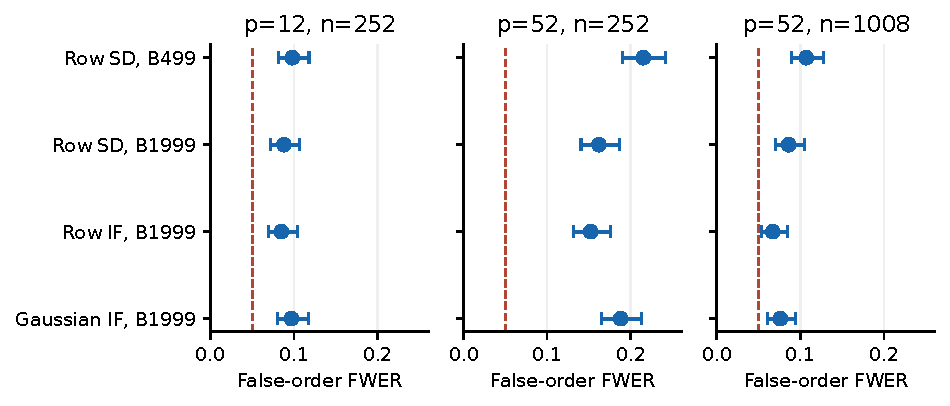
\includegraphics[width=\textwidth]{Fig_audit.pdf}
\caption{False-order FWER in the paired IID audit. Horizontal intervals are individual Wilson Monte Carlo intervals; the vertical line marks 0.05.}\label{fig:audit}\end{figure}



\section{Polish equity sensitivity study}\label{sec:gpw}
Polish stock correlation trees motivate the financial setting \citep{galazka2011}. A frozen historical assembly combines publicly available Bankier price histories, WIG observations and archived GPW index portfolios.\ifanonymous\else\ The input provenance and derived results are archived with immutable version identifiers \citep{previouscode}.\fi\ The base panel contains 231 origins from 2007--2025, each with 252 daily returns and 41--60 eligible stocks. Complete-history, positive-volume and nonzero-return checks are retained. Vendor prices are not certified dividend-inclusive total returns, extraordinary membership changes are not fully reconciled, and missing historical series prevent a complete licensed-market reconstruction.

Three representations---raw returns, cross-sectional demeaning and WIG residualization---use the same 999 circular block-bootstrap draws with block length ten, motivated by dependent resampling \citep{kunsch1989}, giving 693 base analyses. A fixed annual grid adds 466 analyses with nested liquid-stock groups, 252/504/1008-session lookbacks and block-length checks. These target Pearson trees and serially dependent returns. Their interpretation is sensitivity and temporal stability, separate from the exact Kendall IID applications above. Weekly or monthly nonoverlapping returns would not by themselves establish IID sampling.

Across matched stock groups, increasing the lookback from 252 to 1008 sessions reduces mean degree width by 13.9\%, 14.1\% and 10.3\% for groups of 10, 20 and 40 stocks. All rank ranges remain $[1,p]$. All 81 exclusions from the planned primary grid and 51 unavailable primary forward configurations per representation are retained. Full panel results, forward summaries and independent checks of 109,548 improving rational certificates appear in the supplement. This case study identifies a resolution limitation; it does not validate nominal bootstrap coverage for financial time series.

\section{Complete Polish-market sensitivity summaries}
\begin{table}[htbp]
\caption{All 231 windows per representation. Widths are averages of the within-window mean degree width. Full ranks is the mean fraction of vertices with interval $[1,p]$. Hubs counts certified unique hubs over all windows. These are nominal bootstrap diagnostics.}\label{tab:gpw}
\centering\small
\begin{tabular}{lrrrr}
\toprule
Representation & Minor width & Path-LP width & Full ranks & Hubs \\
\midrule
Raw & 49.89 & 45.99 & 1.00 & 0 \\
Demeaned & 49.90 & 46.51 & 1.00 & 0 \\
WIG residual & 49.91 & 47.63 & 1.00 & 0 \\
\bottomrule
\end{tabular}
\end{table}
The refined projection reduces the raw-network mean degree width from 49.89 to 45.99, a 7.8\% reduction relative to the minor. It does not resolve hub ranks: all 35,979 reported vertex--window--representation rank intervals remain $[1,p]$. No unique hub and no top-decile membership is certified. There are 85,129 saved rational certificates for improved degree or anchor-contrast endpoints. These improvements demonstrate a stricter feasible-set projection, but not an informative financial hub ranking.

The all-ranks result is specific to these windows, this calibration and these outer projections. It does not prove that no population hub exists or that no other statistically justified procedure could identify one. It also does not validate the nominal error rate: the calibration failures in Table~\ref{tab:bootstrap} remain relevant.

\subsection{Longer windows, nested liquid universes and forward diagnostics}\label{sec:extended}
The full-panel result motivates a sensitivity analysis that separates sample length from changing stock composition. Before computing the extended outcomes, we fixed the last recorded origin in every represented calendar year, giving 19 annual origins. The complete retrospective sensitivity grid and its unavailable cases are reported. At each origin, we use the longest calendar-available lookback from 504 and 1008 sessions to screen the original eligible list. Eligibility requires complete past returns, supplied prices and volumes, positive volume on at least 90\% of sessions, at most 15\% zero returns, and positive variance. Within this eligible set we rank stocks by median supplied closing price times volume, breaking ties by ISIN. This is an available-data liquidity proxy, not a certified corporate-action-adjusted traded-value measure.

We take nested groups of 10, 20 and 40 stocks. Their membership is kept fixed when comparing 252, 504 and 1008 sessions at the same origin. Changing group size changes the population tree target; a hub of a small liquid subnetwork need not be a hub of the full market. Demeaning is recomputed within each selected group, while factor residualization retains the same WIG series. All dated observations used for selection precede or coincide with the origin; future observations never enter selection. Vendor histories can incorporate later revisions, so this rule does not establish a fully point-in-time data source.

Of 513 planned origin--lookback--group--representation combinations, 81 cannot be evaluated because of insufficient calendar history or too few eligible stocks. We retain the full exclusion list. The remaining 432 primary analyses use block length ten and 999 common-row resamples per origin and lookback, across all three representations. A further 34 raw-network analyses examine block lengths five and twenty at $p=20,n=1008$, for all 17 available origins. These are nominal, per-configuration bootstrap projections. We do not claim simultaneous coverage over the grid or valid 95\% coverage for dependent returns.

\begin{table}[htbp]
\caption{Raw-network comparison on identical stocks and matched origins. The 1008-session availability criterion leaves 17 origins for groups of 10 and 20, and ten for groups of 40. Widths and forced-edge counts are within-group origin averages. Full ranks is the fraction of vertex ranges remaining $[1,p]$.}\label{tab:extended}
\centering\small
\begin{tabular}{rrrrrr}
\toprule
$p$ & Origins & $n$ & Degree width & Forced edges & Full ranks \\
\midrule
10 & 17 & 252 & 6.71 & 0.47 & 1.00 \\
10 & 17 & 504 & 6.18 & 0.59 & 1.00 \\
10 & 17 & 1008 & 5.78 & 1.00 & 1.00 \\
20 & 17 & 252 & 15.04 & 0.47 & 1.00 \\
20 & 17 & 504 & 14.14 & 0.65 & 1.00 \\
20 & 17 & 1008 & 12.92 & 1.35 & 1.00 \\
40 & 10 & 252 & 32.82 & 0.00 & 1.00 \\
40 & 10 & 504 & 31.03 & 0.20 & 1.00 \\
40 & 10 & 1008 & 29.45 & 0.80 & 1.00 \\
\bottomrule
\end{tabular}
\end{table}
The matched-origin mean degree width decreases by 13.9\%, 14.1\% and 10.3\% when moving from 252 to 1008 observations for groups of 10, 20 and 40 respectively. More edges are forced under the nominal order region, but none of the 432 primary or 34 block-sensitivity configurations yields a non-full vertex rank interval or a certified unique hub. The negative ranking result therefore survives a fourfold lookback extension, liquidity-based dimension reduction, and the stated block checks. This describes resolution for the stated procedures and targets.

\begin{table}[htbp]
\caption{Block-length sensitivity for the same 17 raw-network origins, $p=20,n=1008$. Resampling seeds differ between block lengths.}\label{tab:blocks}
\centering\small
\begin{tabular}{rrrrr}
\toprule
Block length & Origins & Degree width & Forced edges & Full ranks \\
\midrule
5 & 17 & 12.94 & 1.24 & 1.00 \\
10 & 17 & 12.92 & 1.35 & 1.00 \\
20 & 17 & 12.93 & 1.29 & 1.00 \\
\bottomrule
\end{tabular}
\end{table}
For a forward diagnostic, we hold the training stock group fixed and estimate a new tree using the next 252 sessions. The diagnostic is available only when every selected stock and the factor have complete future returns. We neither impute unavailable histories nor drop a future-missing stock from the selected group. There are 93 complete primary configurations per representation, out of 144; the remaining 51 have incomplete future histories or insufficient follow-up. Overlapping lookbacks and nested groups mean these are not 93 independent samples. Forward summaries are conditional on future-history availability and may be affected by attrition; no reweighting corrects that selection. We compute the fraction of transitive training order statements whose direction agrees with the future correlation estimates, and whether the training anchor remains tied for largest future degree. These are descriptive temporal-stability measures, not population coverage tests or portfolio-performance results.

\begin{table}[htbp]
\caption{Forward diagnostics over the next 252 sessions. Order agreement averages the within-configuration fractions, giving each configuration equal weight. Anchor still top includes ties and does not establish a unique hub.}\label{tab:forward}
\centering\small
\begin{tabular}{lrrr}
\toprule
Representation & Configurations & Order agreement & Anchor still top \\
\midrule
Raw & 93 & 95.7\% & 35/93 \\
Demeaned & 93 & 95.2\% & 19/93 \\
WIG residual & 93 & 93.9\% & 19/93 \\
\bottomrule
\end{tabular}
\end{table}
Estimated edge-order directions persist much more frequently than the identity of the estimated highest-degree vertex. This comparison involves different functionals: preservation of many inequalities is not equivalent to preservation of a hub, and a high fraction of correct directions need not mean that every direction is preserved jointly. Because the population can change over time, the forward sample is not a known-truth coverage benchmark. The calibration failures in Section~\ref{sec:simulation} remain unresolved.

As an illustration, the earliest complete raw-network configuration with anchor bootstrap frequency at least 0.9 and loss of top position in the future sample is the 2008 annual origin, $p=10,n=504$. The anchor is PKOBP; it is tied for highest degree in 91.2\% of bootstrap trees, while its nominal degree range is [1, 9] and rank range is [1, 10]. Its future estimated rank range is [3, 10], despite 100.0\% directional agreement for the certified training orders. The illustration is selected retrospectively by the stated rule; all configurations are reported, and it is not additional confirmatory evidence.

\begin{figure}[htbp]\centering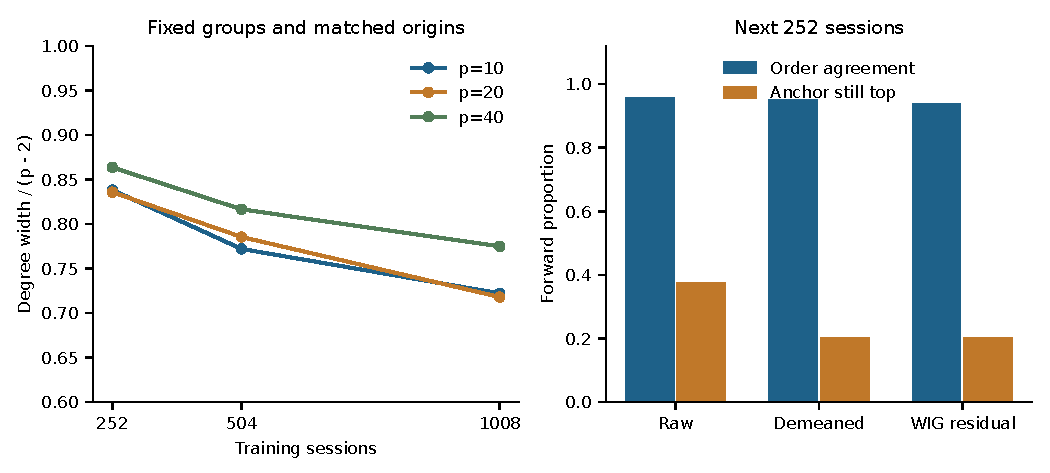
\includegraphics[width=\textwidth]{Fig_empirical.pdf}\caption{Extended empirical diagnostics. Left: mean raw-network degree width divided by $p-2$, on the matched origins and fixed stock groups in Table~\ref{tab:extended}. Right: forward edge-order agreement and retention of the training anchor among the highest-degree vertices, from Table~\ref{tab:forward}. Both panels are descriptive; neither supplies a validated confidence level for GPW returns.}\label{fig:empirical}\end{figure}
Independent verification reconstructs the selection rule for all 50 origin--group universes, checks five source-input hashes and all 9,710 additional vertex records, recomputes the 303 available forward analyses including block sensitivities, and validates all 24,419 improving rational LP certificates. Every check passes. Longer financial windows increase sample size while raising the possibility of regime changes, so their improved degree resolution must be interpreted alongside that stationarity limitation.



\subsection*{Funding}No dedicated funding was received for this study.
\subsection*{Competing interests}The authors declare no relevant competing interests.
\subsection*{Data availability}Derived results, fixed simulation designs, data provenance and verification code accompany the article. The empirical analysis uses the frozen historical data assembly described above. Original UCI measurement files and their CC BY 4.0 attribution are included. Raw third-party stock-price histories are not redistributed; source records and hashes document their availability and limitations.
\subsection*{Code availability}\ifanonymous Reproducibility code and immutable identifiers are supplied separately to the editors.\else The implementation, designs, individual results and certificate verifiers are available at \url{https://github.com/mgalazka84/gpw-hub-reliability/tree/practical-value-v0.6/contrast_inference}.\fi
\subsection*{Declaration of generative AI and AI-assisted technologies in the manuscript preparation process}The authors used ChatGPT/Codex (OpenAI) to assist with writing code. The authors reviewed and tested the code and take full responsibility for the content of the article.
\setlength{\bibsep}{2pt}
\bibliographystyle{plainnat}
\bibliography{references}
\end{document}
